\chapter{Considerações Gerais}
\label{cap:02}

\section{O que é um jogo?}

Segundo o designer de jogos \citeauthorandyear{Crawford1997}, para compreender os jogos e seu design, deve-se primeiramente definir o que se quer representar com a palavra "jogo", a qual ele define como sendo um sistema fechado que representa subjetivamente um subconjunto da realidade. Essa afirmação descreve um jogo como algo completo e autossuficiente, com regras bem definidas que determinam seu funcionamento.

Além disso, o autor identifica quatro elementos fundamentais presentes em todos os jogos. O primeiro é a representação, pois considera que todo jogo sempre reflete, de alguma maneira, aspectos da realidade, mesmo que de forma abstrata ou fantasiosa. O segundo é a interação, pois os jogadores influenciam o jogo ao tomarem decisões. O terceiro é o conflito, que se manifesta por meio de desafios e competição. Por fim, há a segurança, já que as consequências do jogo raramente impactam a realidade.


Já \citeauthorandyear{Suits1978}, filósofo canadense conhecido por seu trabalho sobre a natureza dos jogos, apresenta uma definição mais voltada para o ato de jogar, na qual determina que jogar um jogo é se envolver voluntariamente a uma atividade para alcançar um estado específico, aceitando seguir regras limitantes. Ele também introduz o conceito de \textit{lusory attitude}, que consiste nos jogadores se submeterem a desafios desnecessários para tornar o jogo possível. 



\citeauthorandyear{Crawford1997} define os tipos distintos de jogos, caracterizados a seguir.



\subsection{Jogos de Tabuleiro}

Primeiramente, temos os jogos de tabuleiro, que consistem em uma superfície dividida em setores, os quais são ocupados por um conjunto de peças que, nas configurações comuns, estão diretamente associadas aos jogadores, que as movimentam pelo tabuleiro com o objetivo de capturar as peças do adversário. Um exemplo popular desse tipo de jogo é o Xadrez, que se destaca como um dos jogos de estratégia mais clássicos e influentes, representando bem a essência dos jogos de tabuleiro.

Na Figura~\ref{fig:xadrez}, é ilustrado um tabuleiro de Xadrez com suas peças no começo de uma partida.


\FloatBarrier
\begin{figure}[!htbp]
	\centering
	\caption{Tabuleiro de Xadrez e suas peças}
	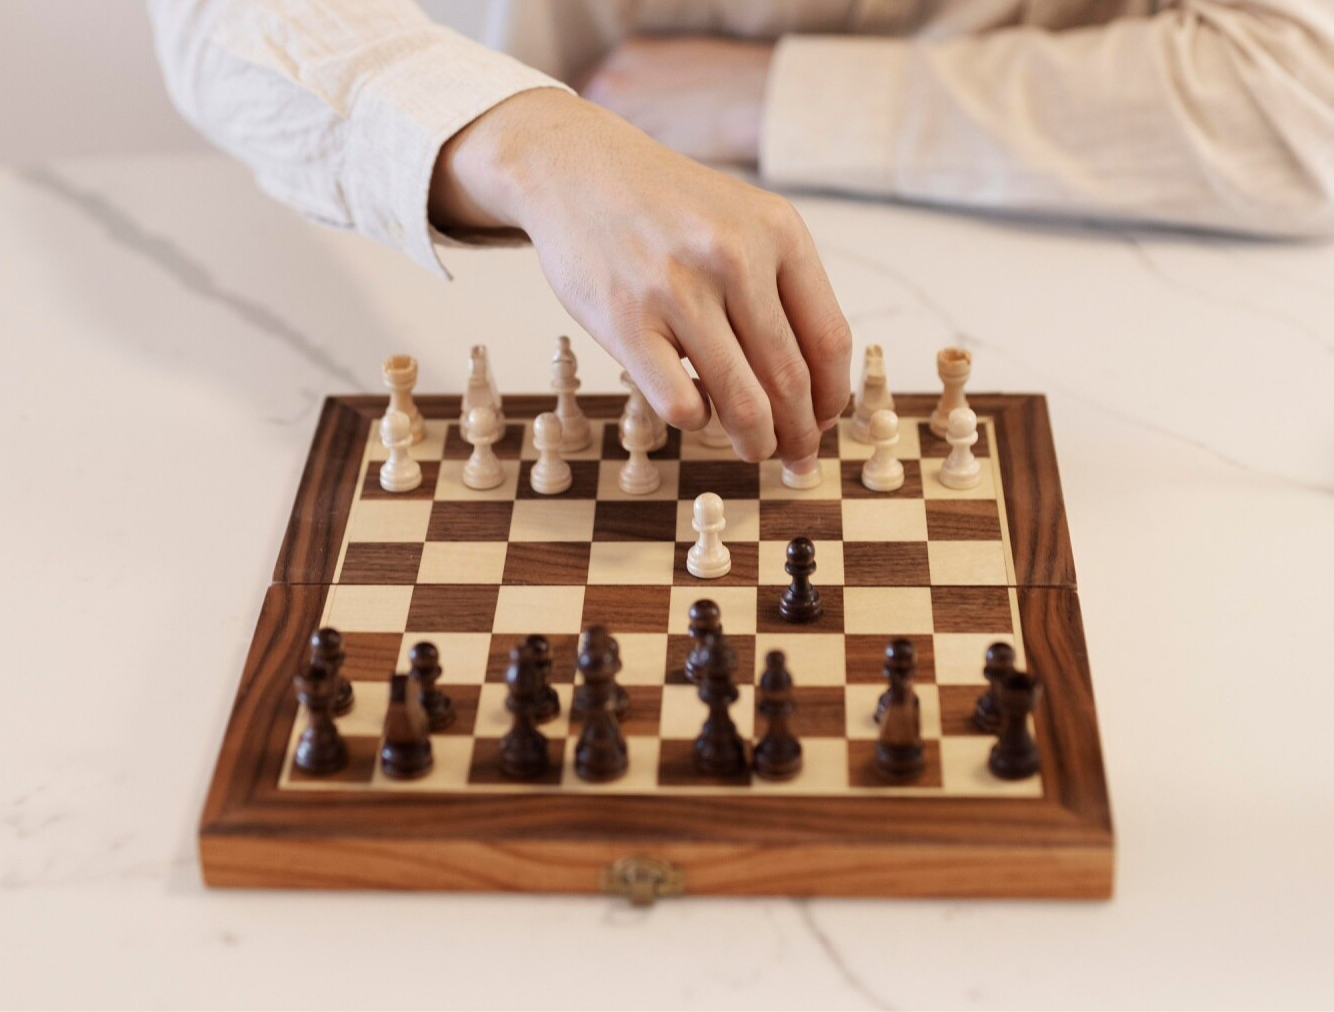
\includegraphics[width=0.7\linewidth]{imagens/Xadrez.png}
	\\\textbf{Fonte:} Freepik
	\label{fig:xadrez}
\end{figure}
\FloatBarrier

\subsection{Jogos de Cartas}

Uma segunda classe de jogos são os jogos de carta, que utilizam um baralho composto por 52 cartas, divididos entre quatro naipes e treze fileiras. O uso do baralho varia conforme o objetivo do jogo, e uma das razões pelas quais os jogos de cartas são tão fascinantes é seu equilíbrio entre sorte e habilidade, diferente dos jogos totalmente aleatórios, como os dados, ou puramente estratégicos, como o xadrez \cite{Parlett1990}.


Segundo \citeauthorandyear{Parlett1990} as cartas possuem uma característica dupla que influencia diretamente a dinâmica dos jogos: a aleatoriedade, que ocorre porque são embaralhadas antes do jogo, e o sigilo, já que apenas o jogador que as possui pode ver seu valor. A questão de sorte nos jogos de cartas está frequentemente ligada à probabilidade, permitindo assim utilizar cálculos matemáticos para prever e influenciar resultados ao longo das partidas. 

Na Figura~\ref{fig:cartas} são apresentadas as cartas presentes em um baralho.


\FloatBarrier 
\begin{figure}[!htbp]
	\centering
	\caption{Cartas de um baralho}
	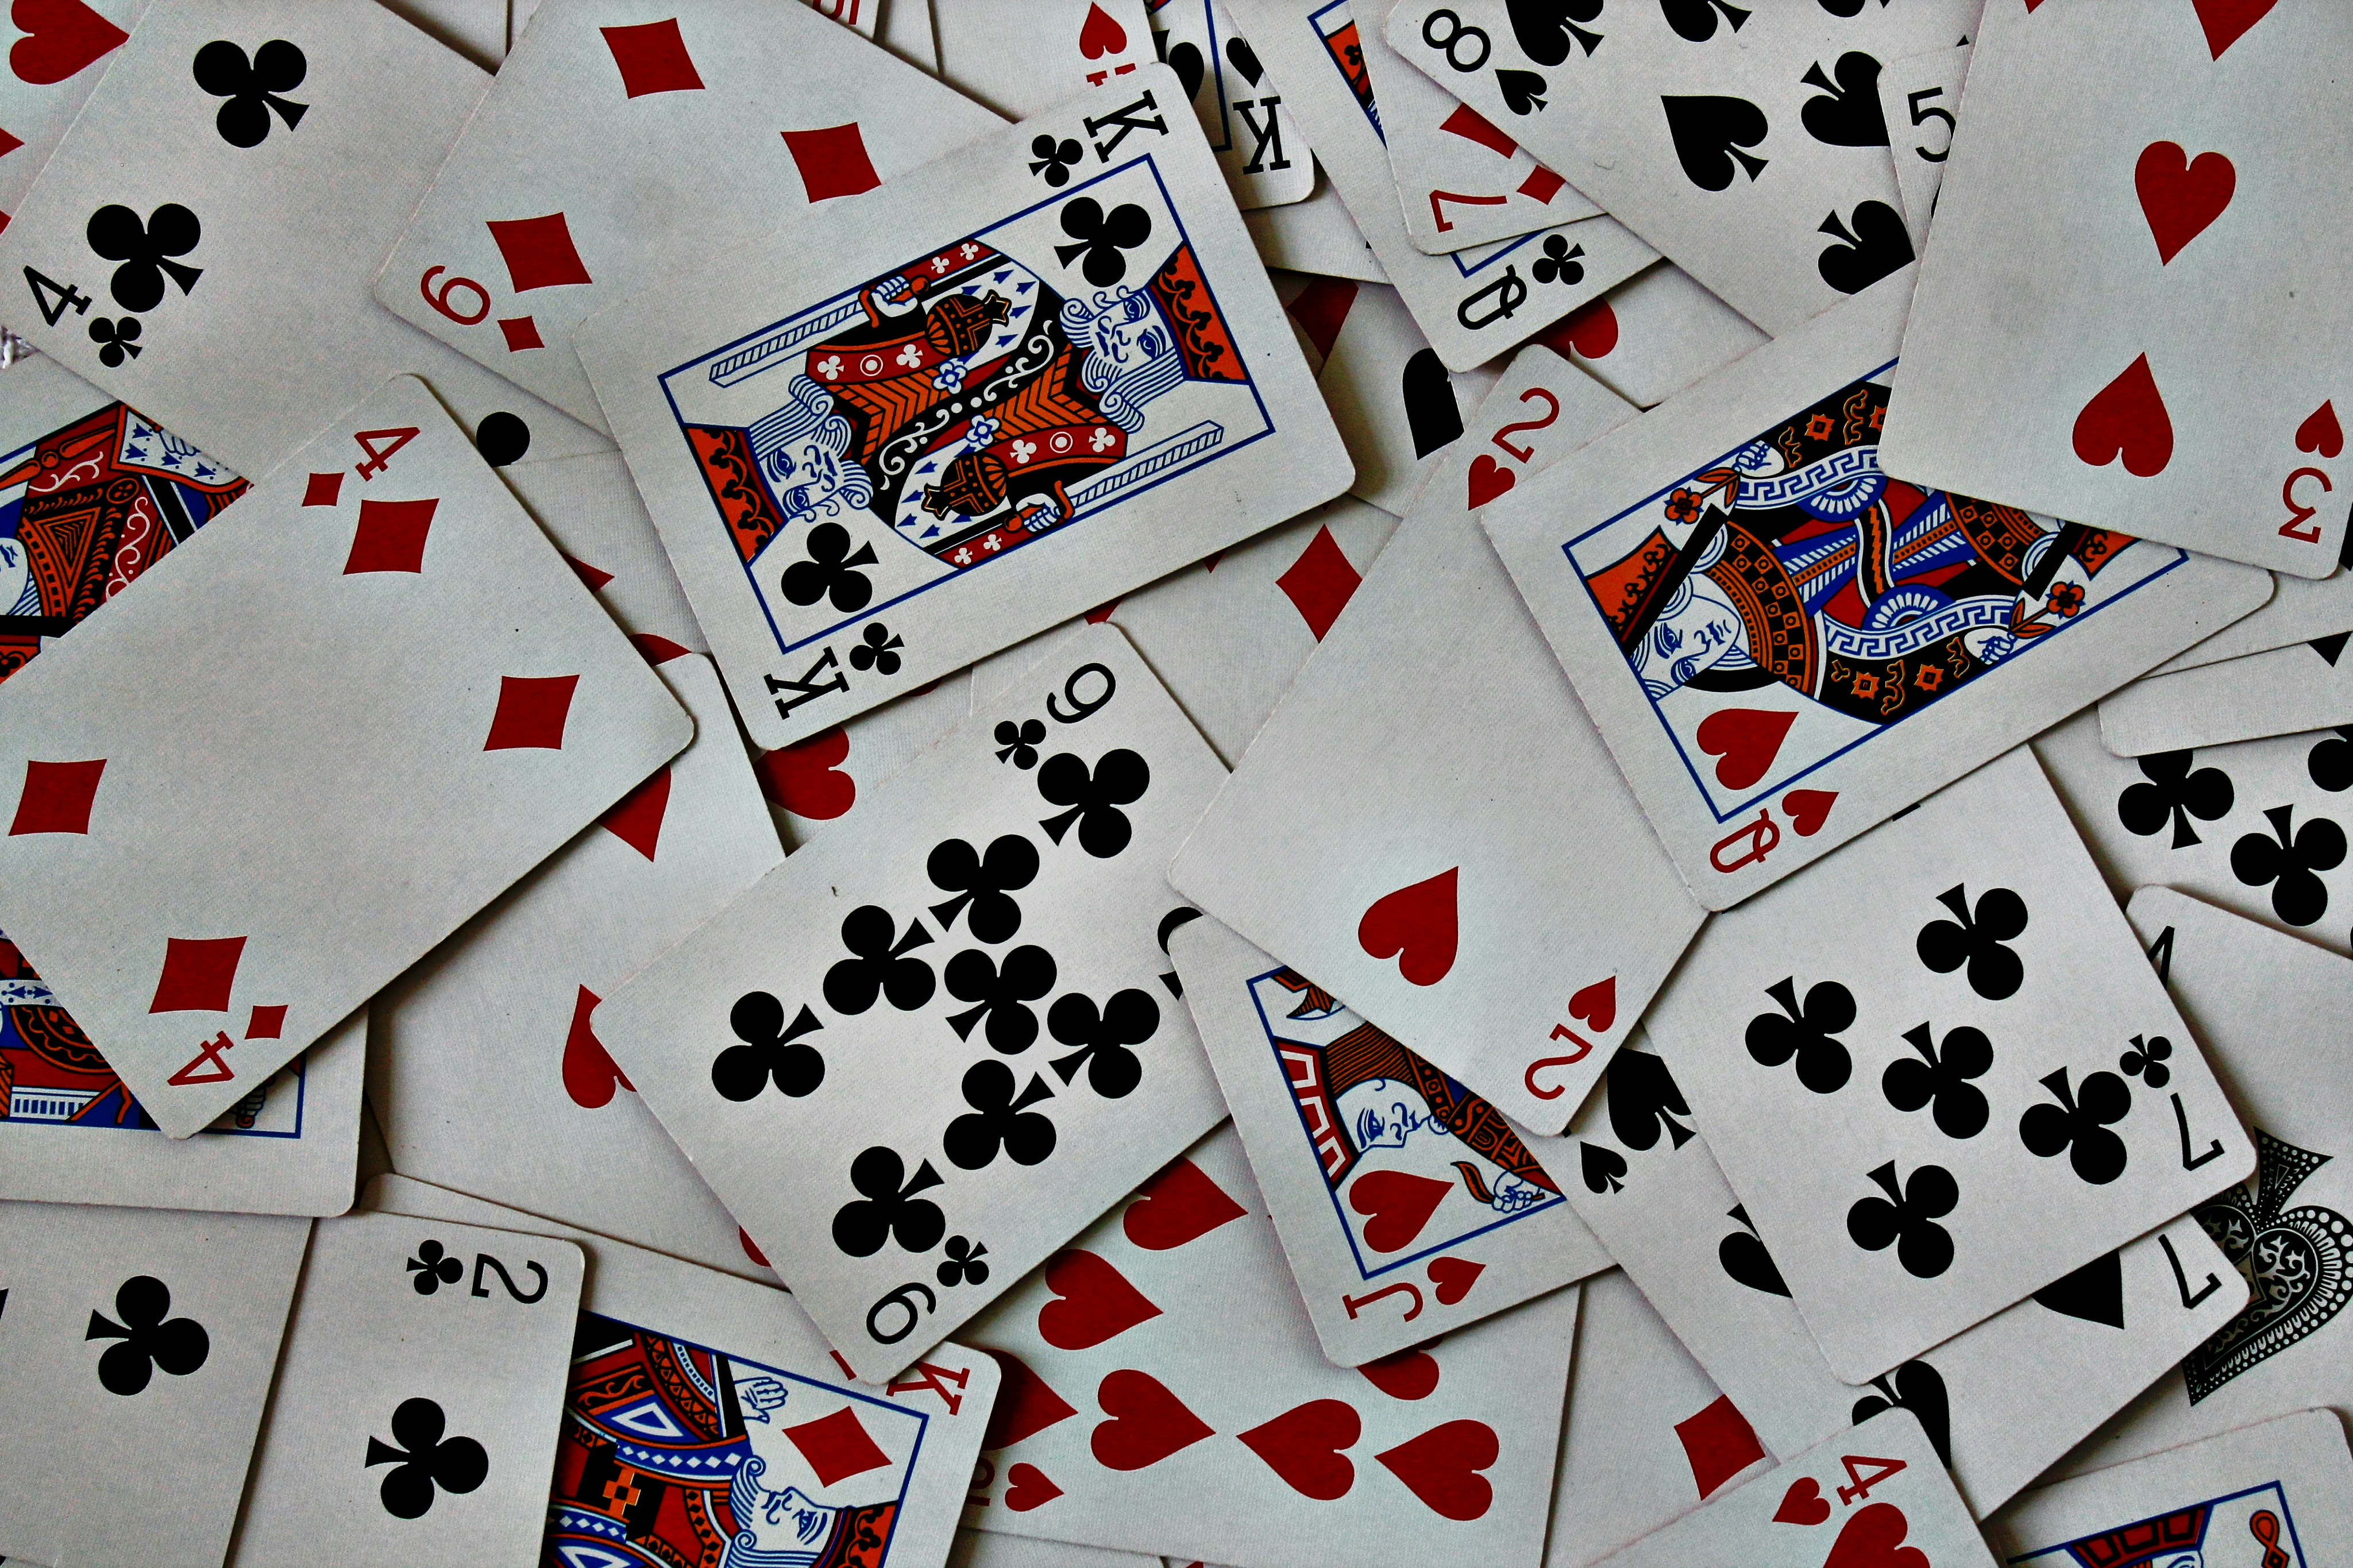
\includegraphics[width=0.7\linewidth]{imagens/Cartas.jpg}
	\\\textbf{Fonte:} https://unsplash.com/pt-br/fotografias/uma-pilha-de-cartas-de-baralho-sentadas-umas-em-cima-das-outras-P787-xixGio
	\label{fig:cartas}
\end{figure}
\FloatBarrier


\subsection{Jogos Atléticos}


Há também os jogos atléticos, uma das formas mais tradicionais de jogos, que destaca a destreza física em detrimento das habilidades mental e possuem regras que especificam estritamente as ações que o jogador pode ou não realizar. Tais jogos estão em uma linha tênue com as competições atléticas, sendo distinguidos pelo grau de interação entre os jogadores \cite{Crawford1997}. Na Figura~\ref{fig:futebol} há um exemplo de jogo atlético, o futebol.


\FloatBarrier 
\begin{figure}[!htbp]
	\centering
	\caption{Jogo de futebol}
	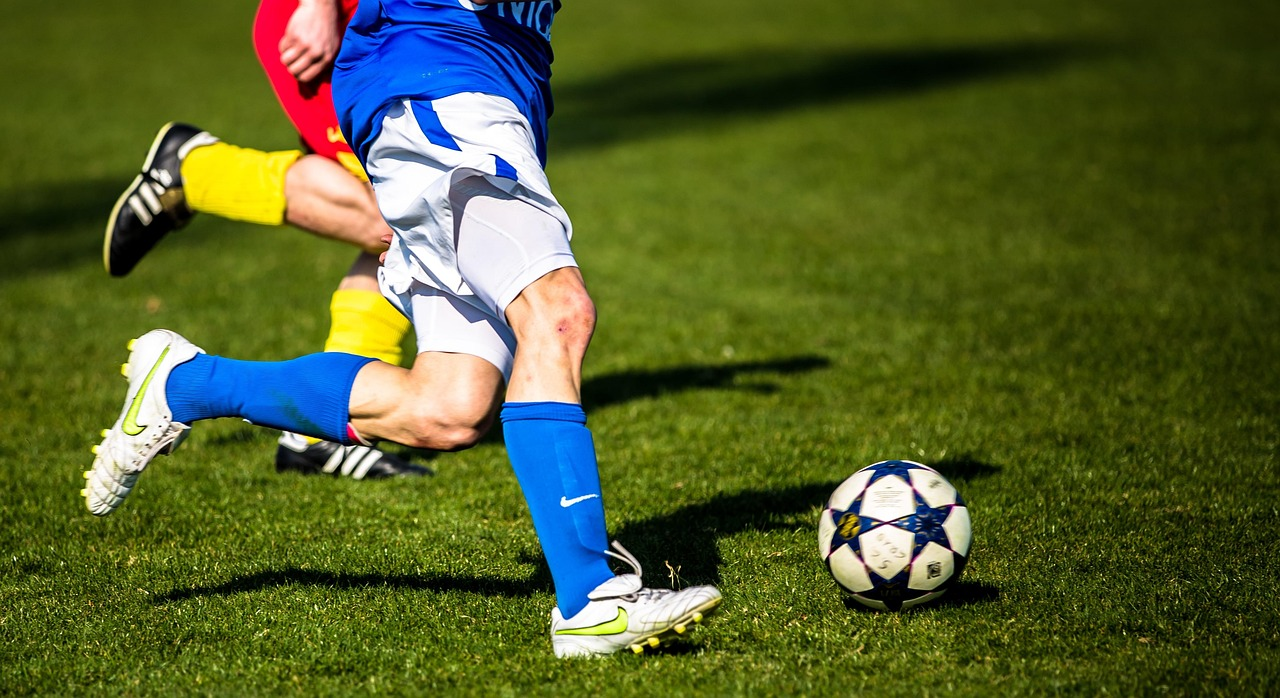
\includegraphics[width=0.7\linewidth]{imagens/futebol.jpg}
	\\\textbf{Fonte:} https://pixabay.com/pt/photos/futebol-duelo-grama-bola-esportes-1331838/
	\label{fig:futebol}
\end{figure}
\FloatBarrier



\subsection{Jogos Digitais}


Por fim, temos os jogos Digitais, os mais populares atualmente e a categoria central deste trabalho. Esses jogos se adequam a diferentes tipos de computadores e plataformas, incluindo máquinas dedicadas, como os fliperamas, consoles domésticos, computadores pessoais e dispositivos portáteis, como o \textit{Nintendo DS} ou até mesmo os celulares \cite{Crawford1997}.


\section{Tipos de Jogos Eletrônicos}

Segundo a definição de \citeauthorandyear{Juul2005}, pesquisador dinamarquês reconhecido na área de \textit{game studies}, os jogos eletrônicos são definidos como uma combinação de regras reais inseridas em mundos fictício, com os quais os jogadores interagem. Essa interação não se limita apenas às mecânicas dos jogos; ela se manifesta em diversos aspectos, incluindo seu design, bem como a forma que os jogos são interpretados, utilizados e discutidos.

No entanto, essa definição desconsidera aspectos culturais nos quais o jogo está inserido, focando apenas na estrutura interna do jogo. E a partir disso, \citeauthorandyear{Apperley2006}, teórico da mídia digital e pesquisador dos estudos de jogos, propõe uma abordagem alternativa, categorizando os videogames com base em como eles são jogados e recebidos. Essa proposta compreende os jogos a partir das práticas sociais e culturais, enfatizando a experiência prática e situada do jogador.

A categorização dos videogames de \citeauthorandyear{Apperley2006} será apresentada a seguir.


\subsection{Simulação}

Embora todos os jogos sejam, de certa forma, simulações, os jogos de simulação buscam representar claramente uma atividade do mundo real, sendo relacionadas a esportes, voos e direção, ou até mesmo simular a dinâmica de cidades e vilarejos. A maior parte desses jogos se encaixam na noção de remediação, pois sua jogabilidade é reaproveitada de atividades relativamente comuns ou representadas nas mídias. Um exemplo popular é o jogo \textit{Euro Truck Simulator}, que simula a direção de um caminhão, apresentada na Figura~\ref{fig:simulacao}.


\FloatBarrier 
\begin{figure}[!htbp]
	\centering
	\caption{\textit{Euro Truck Simulator}}
	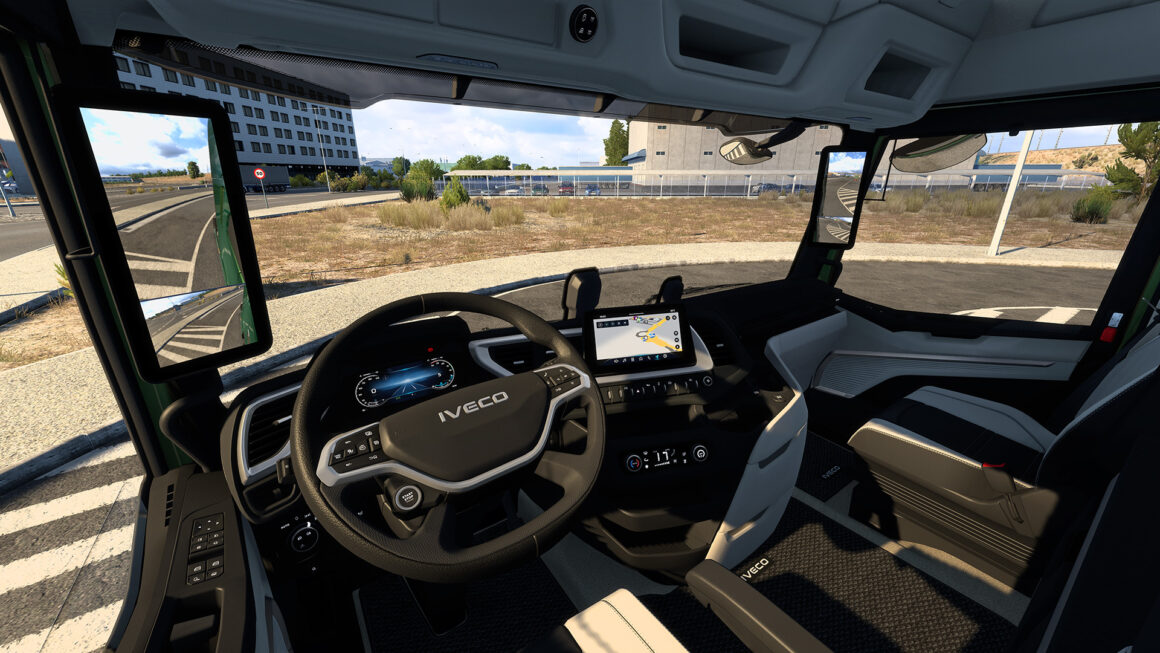
\includegraphics[width=0.7\linewidth]{imagens/EuroTruck.jpg}
	\\\textbf{Fonte:}https://estradao.estadao.com.br/caminhoes/caminhao-pesado-iveco-s-way-estreia-no-euro-truck-simulator-2/ 
	
	\label{fig:simulacao}
\end{figure}
\FloatBarrier


\subsection{Estratégia}

Os jogos de estratégia são caracterizados pelo planejamento e pela tomada de decisões táticas. Geralmente são dividido em dois subgêneros: a estratégia em tempo real (RTS) e baseada em turnos (TBS). Ambos possuem uma estética semelhante, sendo tendentes a um conceito fotorrealista. Tais jogos priorizam a gestão de recursos, o pensamento analítico e a adaptação estratégica, exigindo, assim, uma atenção profunda do jogador. Um exemplo de TBS é o jogo \textit{Teamfight Tactics (TFT)} apresentado na Figura~\ref{fig:tactics}.

\FloatBarrier 
\begin{figure}[!htbp]
	\centering
	\caption{\textit{Teamfight Tactics (TFT)}}
	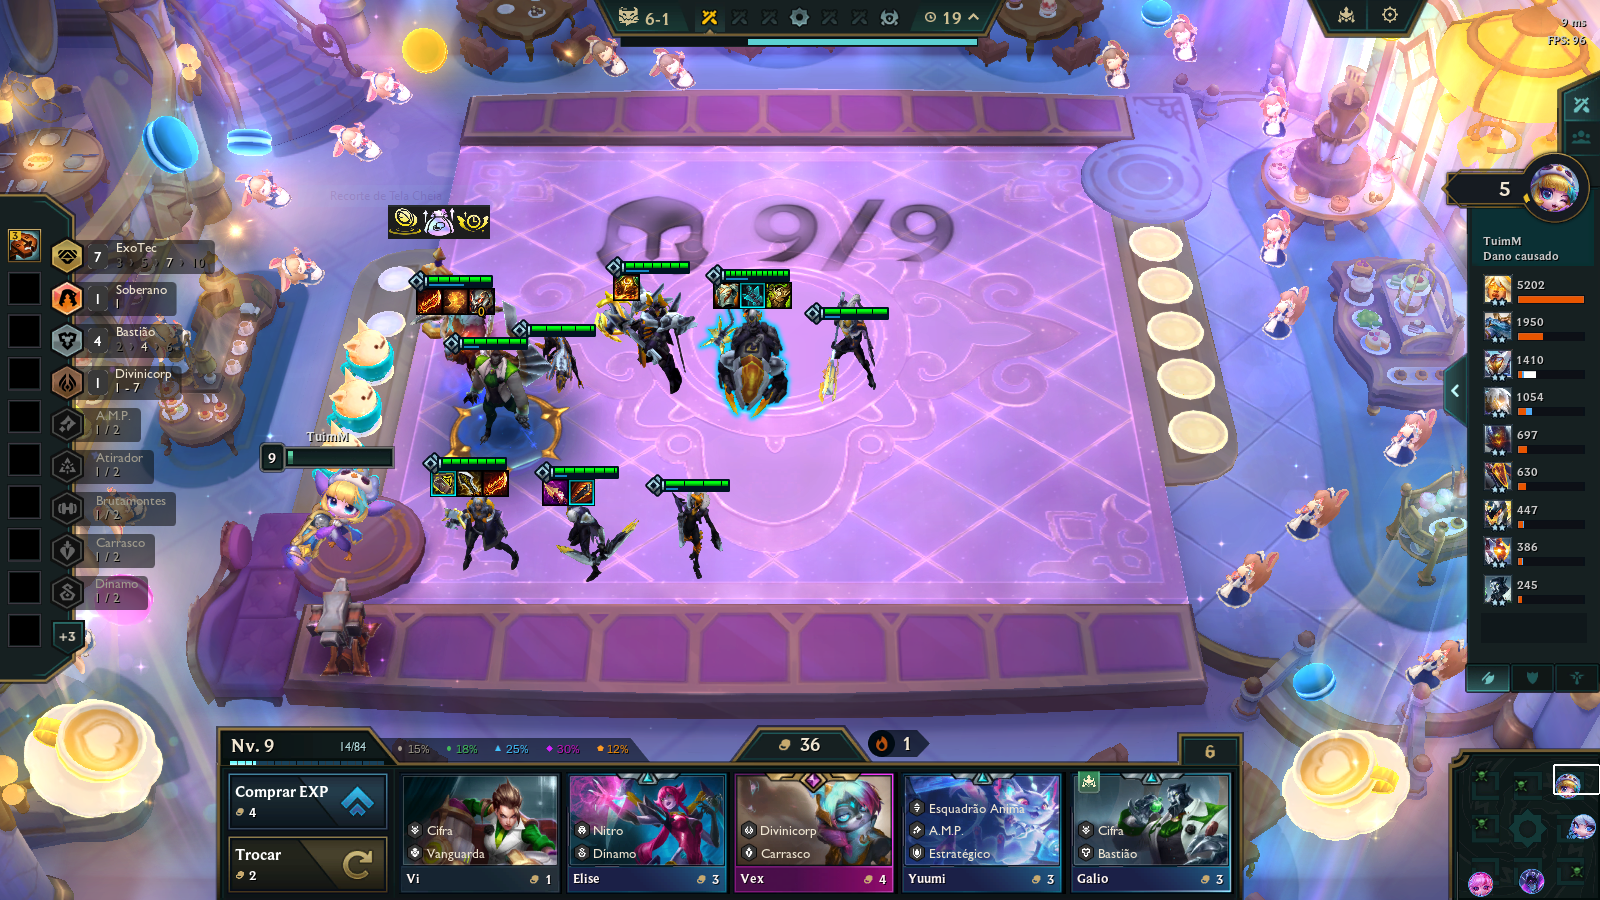
\includegraphics[width=0.7\linewidth]{imagens/tft3.png}
	\\\textbf{Fonte:} Elaborada pelo autor
	
	\label{fig:tactics}
\end{figure}
\FloatBarrier


\subsection{Ação}

Assim como os jogos de estratégia, os jogos de ação também podem ser divididos em dois subgêneros: jogos de tiro em primeira pessoas, conhecidos como FPS (\textit{First Person Shooters}), nos quais a câmera simula a própria visão do jogador, e jogos em terceira pessoa, que representam o personagem totalmente visível na tela, geralmente visto por trás. Tais jogos priorizam a agilidade, precisão e o tempo de reação do jogador, oferecendo experiências intensas e dinâmicas. Um FPS popular é o jogo \textit{Valorant} apresentado na   Figura~\ref{fig:vava}.


\FloatBarrier 
\begin{figure}[!htbp]
	\centering
	\caption{\textit{Valorant}}
	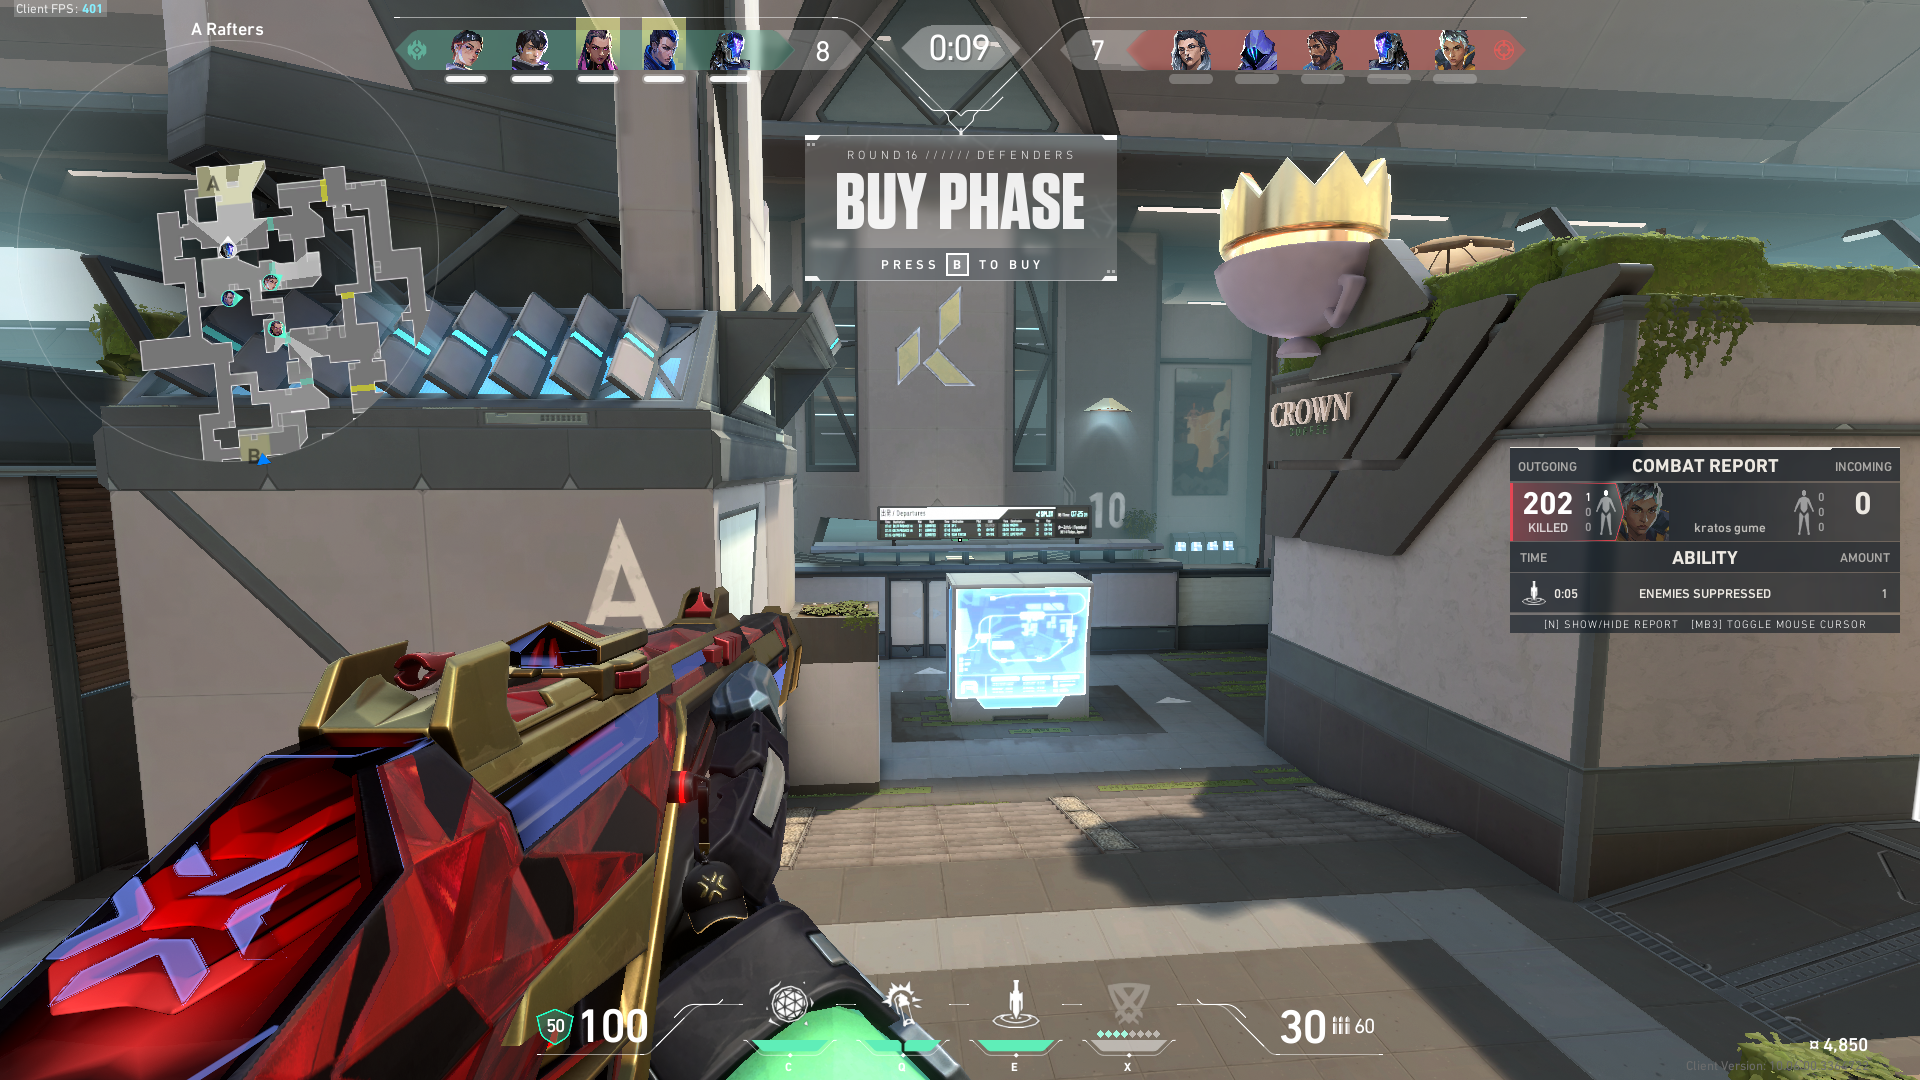
\includegraphics[width=0.7\linewidth]{imagens/valorant.png}
	\\\textbf{Fonte:} Elaborada pelo autor
	
	\label{fig:vava}
\end{figure}
\FloatBarrier


\subsection{\textit{Role-playing}}

Nos jogos de \textit{Role-playing}, ou RPGs, os jogadores interpretam seus personagens em mundos fictícios, narrando suas ações a um mestre, o qual conduz os resultados dessas ações. Originados do clássico  \textit{Dungeons and Dragons} na década de 1970 \cite{Mason2004}, esse jogos evoluíram para versões digitais, mantendo elementos como a progressão de personagens, porém agora limitando a improvisação e focando em desafios mecânicos e uma narrativa mais centrada.

\section{Tecnologias para Desenvolvimento de Jogos} 









Texto das considerações gerais, dividido em subseções.

Este é um exemplo de como usar figuras. Referência cruzada: Figura~\ref{fig:exemplo}

\FloatBarrier
\begin{figure}[!htbp]
	\centering
	\caption{Exemplo de figura}
	%scale redimensiona a figura.
	%1.5 = 150% do tamanho original
	%1 = 100% do tamanho original
	%0.20 = 20% do tamanho original
	
\includegraphics[scale=0.4]{imagens/exemploFigura}
	\\\textbf{Fonte:} Elaborada pelo autor
	\label{fig:exemplo}
\end{figure}
\FloatBarrier


Este é um exemplo de como usar tabelas. Referência cruzada: Tabela~\ref{tab:exemplo}

\FloatBarrier
\begin{table}[!htbp]
	\centering
	\caption{Exemplo de tabela de 2 colunas}
	\begin{tabular}{ c | c }
		\hline
		\textbf{Coluna 1} & \textbf{Coluna 2} \\ \hline
		Dado 1a           & Dado 2a           \\ \hline
		Dado 1b           & Dado 2b           \\ \hline
		Dado 1c           & Dado 2c           \\ \hline
		Dado 1d           & Dado 2d           \\ \hline
	\end{tabular}
	\\ \vspace{0.2cm}
	\textbf{Fonte:} Elaborada pelo autor
	\label{tab:exemplo}
\end{table}
\FloatBarrier


Este é um exemplo de como usar quadros. Referência cruzada: Quadro~\ref{qua:exemplo}

\FloatBarrier
\begin{quadro}[!htbp]
	\centering
	\caption{Exemplo de quadro}
	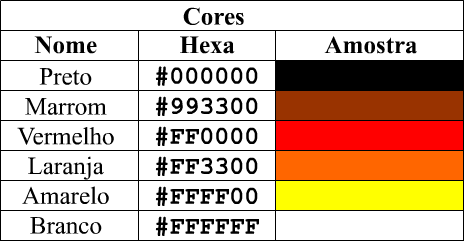
\includegraphics[scale=.7]{imagens/exemploQuadro}
	\\\textbf{Fonte:} Elaborada pelo autor
	\label{qua:exemplo}
\end{quadro}
\FloatBarrier


Este é um exemplo de como usar equações. Referência cruzada: Equação~\ref{eq:exemplo}

\begin{equation}
\sum_{i=1}^{n} i = \frac{n(n+1)}{2}
\label{eq:exemplo}
\end{equation}


Exemplo de inserção de lista de código fonte:

\lstinputlisting[language=Java]{fontes/ClasseExemplo.java} 



Este é um exemplo de como inserir texto sem formatação (ambiente verbatim):

\begin{verbatim}
Texto sem formatação, como espaçamento igual.
\end{verbatim}


Exemplo de lista de itens:

\begin{itemize}
	\item \textbf{Item 1:} texto...;
	\item \textbf{Item 2:} texto...;
	\begin{itemize}
		\item \textbf{Subitem:} texto...;
		\item \textbf{Subitem:} texto...;
		\item \textbf{Subitem:} texto...;
	\end{itemize}
	\item \textbf{Item 3:} texto...;
	\item \textbf{Item n:} texto....
\end{itemize}


Exemplo de lista numerada:

\begin{enumerate}
	\item \textbf{Item:} texto...;
	\item \textbf{Item:} texto...;
	\begin{enumerate}
		\item \textbf{Subitem:} texto...;
		\item \textbf{Subitem:} texto...;
		\item \textbf{Subitem:} texto...;
	\end{enumerate}
	\item \textbf{Item:} texto...;
	\item \textbf{Item:} texto....
\end{enumerate}


Exemplos de comandos para texto e referências:

\begin{itemize}
	\item Para iniciar um novo parágrafo, basta deixar uma linha em branco no código fonte;
	\item Não force o compilador a pular mais de uma linha, pois terá influência negativa na composição do documento;
	\item Sempre deixe o \LaTeX\ realizar a formatação de parágrafos e posicionamento de elementos;
	\item Utilização de aspas simples (abertura \verb|`|, fechamento \verb|'|): `Texto entre aspas simples';
	\item Utilização de aspas duplas (abertura \verb|``|, fechamento \verb|''|): ``Texto entre aspas duplas'';
	\item Negrito (comando \verb|\textbf|): \textbf{texto em negrito};
	\item Itálico (comando \verb|\textit|): \textit{texto em itálico};
	\item Sublinhado (comando \verb|\underline|): \underline{texto sublinhado};
	\item Negrito e itálico (usar comandos juntos): \textbf{\textit{texto em negrito e itálico}};
	\item Alterar cor do texto (comando \verb|\textcolor{cor}{texto}|):
	\begin{itemize}
		\item Exemplo \verb|\textcolor{red}{texto}|: \textcolor{red}{texto vermelho};
		\item Exemplo \verb|\textcolor[RGB]{255, 102, 0}|: \textcolor[RGB]{255, 102, 0}{texto laranja};
		\item Exemplo \verb|\textcolor[HTML]{006AD7}|: \textcolor[HTML]{006AD7}{texto azul};
	\end{itemize}
	\item Ambiente matemático inline (comando \verb|$ expressão $|): $s = x^2-2x +1$;
	\item Referência normal (comando \verb|\cite|):


Exemplo de nota de rodapé\footnote{Essa é uma nota de rodapé!}.


\section{Trabalhos Correlatos}

Pesquise e descreva no mínimo três trabalhos correlatos ao seu.

\subsection{Trabalho 1}

Texto...

\subsection{Trabalho 2}

Texto...

\subsection{Trabalho 3}

Texto...
